\documentclass{article}
\usepackage[utf8]{inputenc}
\usepackage{amsmath}
\usepackage{amsfonts}
\usepackage{amsthm}
\usepackage{geometry}
\usepackage{tikz}
\usetikzlibrary{arrows.meta,
                chains,
                positioning,
                shapes.geometric
                }
\geometry{a4paper, portrait, margin=1in}

\theoremstyle{plain}
\newtheorem{thm}{Theorem}

\theoremstyle{definition}
\newtheorem{defn}{Definition} % definition numbers are dependent on theorem numbers
\newtheorem{exmp}{Example} % same for example numbers

\title{Data Analytics (UE18CS312)\\
\large Unit 1}
\author{Aronya Baksy}
\date{August 2020}

\begin{document}

\maketitle

\section{Introduction}

\begin{defn}
    Interpretation and exploration of past data is known as \textbf{Analysis} of Data
\end{defn}

\begin{defn}
    Data \textbf{Analytics} involves analysis (as defined above) along with predictive modelling of the future from the derived insights
\end{defn}

Data Analytics is a set of statistical and operation research techniques, AI, IT and management strategies used to frame a problem, collect data and use the data to generate insghts that create value for organizations. 

\subsection{Types of Data Analytics}

\begin{enumerate}
    \item \textbf{Descriptive:} Answers the question "What is happening?". Using visualizations effectively, build them using comprehensive, accurate and live data.
    
    \item \textbf{Diagnostic:} Answers the question "Why is it happening?". Identify the root cause and isolate confounding factors
    
    \item \textbf{Predictive:} Answers the question "What will happen?". Predict the outcome of a certain action given the historical data.
    
    \item \textbf{Prescriptive:} Answers the question "What do I need to do?". Recommend strategies and actions based on outcomes of prediction and testing various strategies. 
\end{enumerate}

\subsection{Steps in Data Analytics}

\begin{enumerate}
    \item Data Collection
    
    \item Data Preprocessing
    
    \item EDA
    
    \item Insights (ML/DL)
    
    \item Visual Report
\end{enumerate}
\begin{figure}[h]
    \centering
    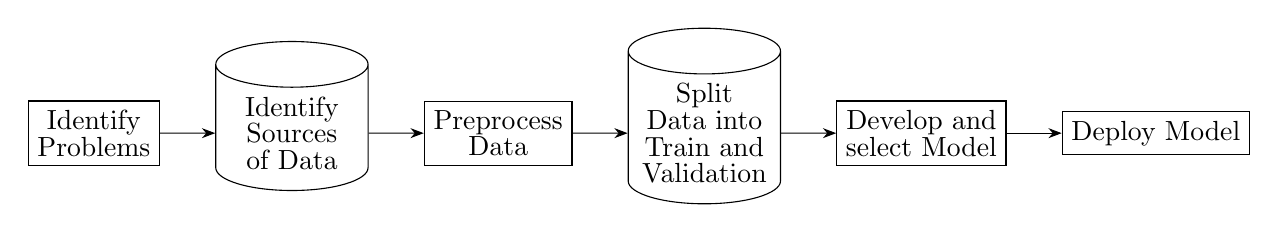
\begin{tikzpicture}[node distance = 5mm and 7mm,
          start chain = going right,
     disc/.style = {shape=cylinder, draw, shape aspect=0.3,
                    shape border rotate=90,
                    text width=17mm, align=center, font=\linespread{0.8}\selectfont},
      mdl/.style = {shape=ellipse, aspect=2.2, draw},
      alg/.style = {draw, align=center, font=\linespread{0.8}\selectfont}
      ]
    \begin{scope}[every node/.append style={on chain, join=by -Stealth}]
        \node (n1) [alg] {Identify\\Problems};
        \node (n2) [disc] {Identify Sources of Data};
        \node (n3) [alg] {Preprocess \\ Data};
        \node (n4) [disc] {Split Data into\\Train and Validation};
        \node (n5) [alg] {Develop and\\select Model};
        \node (n6) [alg] {Deploy Model};
    \end{scope}
    \end{tikzpicture}
    \caption{Data Analytics Pipeline}
\end{figure}

\subsection{Costs in Business Decision Making}
\begin{itemize}
    \item \textbf{Decision Cost:} Cost of producing a decision, using the help of a decision maker or a fixed procedure.
    \item \textbf{Implementation Cost:} Cost of actions based on the decision taken
    
    \item\textbf{Failure Cost:} Cost of organization's inability to produce and implement the decision. 
\end{itemize}
The aim of data analytics is to reduce these costs. 

\subsection{Business use cases for Data Analytics}
\begin{itemize}
    \item \textbf{Process Improvement:} Reduce cheque clearance time in banks, reduce patient discharge time in hospitals, reduce wastage in manufacturing, reduce time to deliver customer orders in e-com. 
    
    \item \textbf{Problem Solving:} Reduce the impact of NPAs in financial investments, predict financial fraud, reduce inventory management cost in manufacturing, space allocation and route planning in e-com. 
    
    \item \textbf{Decision Making:} Approve loan decisions, decide interest rates, introduce new products, markdown pricing and promotions in e-com.
    
\end{itemize}

\section{Data Sources and Representation}
\subsection{What is Data}
\begin{itemize}
    \item Collection of \textbf{objects} and their \textbf{attributes}.
    
    \item Attributes are the descriptive properties/characteristics of an object. 
    
    \item A single object can also be referred to as a point, an entity, a record, an instance, a sample or a case. 
    
    \item Attribute values are the actual values assigned to an attribute for a particular object. They could be alphanumeric, ordinal, symbols, etc. 
    
    \item The same attribute can be mapped to different attribute values. The set of all unique values that an attribute can take is called the \textbf{domain} of that attribute. 
    
    \item Different attributes may be mapped to the same attribute value, but with different meanings and properties. (eg: ID number and age are both integers but mean entirely different things).
\end{itemize}

\subsection{Types of Data}
\begin{itemize}
    \item Based on \textbf{measurement level}:
    \begin{enumerate}
        \item \textbf{Nominal:} Also known as categorical attributes, represent the names of different states or groups. There is no order or rank among these categories. (eg: ID numbers, names, ZIP codes, eye colours)
            
        \item \textbf{Ordinal:} The values have an inherent ranking but no absolute value of their own. (eg: Grades, height (tall/medium/short), taste of chips on a scale of 1-10)
            
        \item \textbf{Interval:} The distance between attribute values is important and carries meaning to the attribute, but their ratio does not mean anything. (eg: Calendar dates, 
            temperatures in C/F) 
            
        \item \textbf{Ratio:} The ratios between different values carries meaning, and there is an absolute zero (eg: length, counts, temperature in K, elapsed time)
    \end{enumerate}
    
    \item Based on \textbf{continuity}:
    \begin{enumerate}
        \item \textbf{Discrete:} Finite/countably infinite set of values, can be represented as integers.
        
        \item \textbf{Continuous:} Real numbers as attribute values, represented as float point numbers.
    \end{enumerate}
\end{itemize}

\subsection{Data Representations}
\subsubsection{Structured and Unstructured Data}
\begin{itemize}
    \item \textbf{Structured} data is data that is represented in rectangular, or matrix form with labelled rows and columns. (eg: Relational Databases, spreadsheets)
    
    \item \textbf{Unstructured} data has no rectangular or matrix representation (eg: text, photos, videos, audio, real-time instrument data, webpages)
    
    \item \textbf{Semi-Structured} data has no rectangular form, but follows some fixed format.
    (eg: XML files, NoSQL databases, e-mails)
\end{itemize}

\subsubsection{Data Cubes}
\begin{itemize}
    \item Data cubes are a method of displaying 3 dimensional data efficiently. They are also called \textbf{OLAP} cubes.
    
    \item They support different analytical operations, called \textbf{OLAP} operations (OnLine Analytical Processing). 
    
\end{itemize}
\begin{figure}[h]
    \centering
    \includegraphics[scale=0.2]{da1.png}
    \caption{A data cube}
    \label{fig:my_label}
\end{figure}

\subsection{OLAP Operations}
\begin{enumerate}
    \item \textbf{Roll-up:} Summarize data by climbing hierarchy or reducing dimension (eg: change cities to countries by grouping all the cities)
    
    \item \textbf{Drill-down:} Increase level of granularity along one axis of the cube. (eg: change time in quarters (Q1, Q2 etc.) to time in months) 
    
    \item \textbf{Slice/Dice:} Projection and Selection (A \textbf{slice} represents the result of a single boolean condition on the cube, eg: \texttt{city == "Toronto"}, while a \textbf{dice} represents the result of a conjunction of 2 or more boolean expressions, eg: \texttt{(city == "Toronto") and (time=="Q1" or "Q2") and (product=="phone" or "laptop") }
    
    \item \textbf{Pivot:} Change the axes of the cube by rotating them. 
\end{enumerate}

\section{Data Exploration}

\begin{itemize}
    \item Data Exploration is used to give basic insights on the patterns present in the data, and its overall shape and distribution. 
    
    \item Exploratory Data Analysis (EDA) consists of using \textbf{summary statistics} and \textbf{data visualization} to derive this information. 
    
    \item The \textbf{population} is defined as the set of all possible observations in a given problem context for which conclusions are to be drawn.
    
    \item The \textbf{sample} is a subset of the population which is of interest to the observer, and based on whom conclusions about the entire population will be drawn. 
\end{itemize}

\subsection{Summarizing Data}
\subsubsection{Measures of Central Tendency}
\begin{itemize}
    \item \textbf{Mean}: Arithmetic average of all the data values.
    \begin{equation}
        \overline{x} = \frac{x_1 + x+_2 + x_3 + ... + x_n}{n} = \frac{1}{n}\sum_{i=1}^{n} x_i
    \end{equation}
    
    The symbol $\overline{x}$ is used to denote the sample mean, and the symbol $\mu$ is used to denote the population mean. 
    
    \item \textbf{Mode}: The most frequently occurring data value. It can be applied to categorical data as well, unlike mean and median.
    
    \item \textbf{Median}: The value that divides the data into two equal parts, with half the data below and the other half above the median. 

\end{itemize}

\subsubsection{Measures of Spread}
\begin{itemize}
    \item \textbf{Quartiles}: The first ($Q_1$), second ($Q_2$) and third ($Q_3$) quartiles divide the data into 4 equal parts. The second quartile is the median.\\
    The kth quartile can be calculated using the value at the index $i$ given by
    
    \begin{equation}
        i = k \frac{n+1}{4}
    \end{equation}
    
    The \textbf{IQR} (interquartile range) is defined as the part of the data where the middle 50\% of the data lies. It is calculated as $Q_3 - Q_1$
    
    \item \textbf{Percentiles}: This is a further generalization of the quartile, where the data is broken into 100 equal parts. The quartiles are the 25th, 50th and 75th percentiles respectively.\\
    The kth percentile can be calculated as the data value at the index $i$ given by 
    \begin{equation}
        i = k \frac{n+1}{100}
    \end{equation}
    
    \item \textbf{Variance}: Measure of variability of the data points from the mean value.
    It is calculated by
    \begin{equation}
        \sigma^2 = \frac{1}{n}\sum_{i=1}^{n} (X_i - \mu)^2
    \end{equation}
    The above formula denotes the population variance. The sample variance is calculated as
    \begin{equation}
        s^2 = \frac{1}{n-1} \sum_{i=1}^{n} (X_i - \overline{x})^2
    \end{equation}
    
    The replacement of $n$ with $n-1$ for the sample variance formula is called the Bessel's correction, and is used to correct for the bias that occurs when taking a sample from the population. 
    
    \item \textbf{Standard Deviation}: The amount of dispersion or variance in a dataset is denoted by its standard deviation $\sigma$ or $s$ (population and sample values). 
    It is calculated by taking the \textbf{square root} of the \textbf{variance}. 
\end{itemize}

\subsubsection{Degrees of Freedom}
The number of independent variables in a model, or independent observations in a data set is called the degrees of freedom.\\
Given a sample mean $\overline{x}$ and $n-1$ values, the last value can have only one fixed value, and hence is dependent on the rest of the values. Hence here there are $n-1$ degrees of freedom.\\
If there are $n$ items in the sample and $k$ parameters estimated from the sample, then the number of degrees of freedom is $n-k$

\subsubsection{Chebyshev's Inequality}
The probability of finding a randomly selected value $X$ from the data in the interval $\mu \pm  k \sigma$ is given as:
\begin{equation}
    P(\mu - k\sigma \leq X \leq \mu + k\sigma ) \geq 1 - \frac{1}{k^2}
\end{equation}

\subsubsection{Skewness and Kurtosis}
\begin{itemize}
    \item \textbf{Skewness} is a measure of the symmetry of the distribution. For data to be symmetrical, there must be an equal proportion of data in the intervals $(\mu - k\sigma, \mu)$ and $(\mu, \mu + k\sigma)$, where $k$ is a positive integer. 
    
    \item The skewness is the third moment of the centered distribution of $X$ about the mean $\mu$.
    \begin{equation}
        g_1 = \mathbb{E}\left[ \left(\frac{X - \overline{X}}{\sigma} \right)^3 \right] = \frac{1}{\sigma^3} \frac{\sum_{i=1}^{n} (X_i - \overline{X})^3}{n} 
    \end{equation}
    
    \item For $g_1 > 0$, the tail of the data is longer on the right (+ve dir), for $g_1 < 0$ the tail of the data is longer on the left (-ve dir), while for $g_1 = 0$ both tails are equal. 
    
    \begin{figure}[h]
        \centering
        \includegraphics{da2.png}
        \caption{Positively and Negatively Skewed Distributions}
        \label{fig:my_label_2}
    \end{figure}
    
    \item \textbf{Kurtosis} is a measure of how heavy the tails of a distribution are. It is given by
    
    \begin{equation}
        kurtosis = \mathbb{E}\left[ \left(\frac{X - \overline{X}}{\sigma} \right)^4 \right] = \frac{1}{\sigma^4} \frac{\sum_{i=1}^{n} (X_i - \overline{X})^4}{n}
    \end{equation}
    
    \item A kurtosis value of $<3$ indicates a platykurtic disttribution, $>3$ indicates a leptokurtic distribution while a mesokurtic distribution (eg: the standard normal) has a kurtosis value of 3. 
    
    \item The deviation of a distribution from the standard normal is reflected in the \textit{excess kurtosis}, given by $kurtosis - 3$.
\end{itemize}

\section{Sampling techniques}
\subsection{Probabilistic Sampling}
\begin{itemize}
    \item \textbf{Systematic Sampling}: Picking every $k$th sample, where $k$ is called the sampling rate. (eg: time series analysis, sampling video frames, pixels in an image)
    
    \item \textbf{Simple Random Sampling}: Can be done with replacement (for finite population) or without replacement (infinite or very large population).
    
    \item \textbf{Stratified Sampling}: Divide the data into homogenous sub-groups (called strata) and perform simple random sampling on each sub group. Division into strata is based on some characteristic (eg: income level, address, etc.)
    
    \item \textbf{Cluster Sampling}: Divide the population into clusters, and sample these clusters. Clusters must be internally as heterogenous as possible but two clusters must be similar in their structure. (eg: geographical surveys)
\end{itemize}

\subsection{Non-Probabilistic Sampling}
\begin{itemize}
    \item \textbf{Convenience Sampling}: Pick samples that are convenient to the one running the experiment
    
    \item \textbf{Judgement Sampling}: Pick best samples as per the \textbf{judgement} of the person running the experiment. 
\end{itemize}

\section{Data Visualizations}
\subsection{Histogram}
\begin{itemize}
    \item Used to visualize the frequency distribution of continuous data. 
    
    \item It is the frequency distribution of the data arranged in consecutive non-overlapping intervals. 
    
    \item The area of each rectangle indicates its frequency. If all the bins have same width then height is proportional to frequency. 
    
    \item Histograms can effectively show both skew and kurtosis.
    
    \item Choosing the appropriate bin size is important. Too small a bin size leads to too much noise, while too large a bin size leads to details being overlooked.
    
    \item The histogram of cumulative probabilites represents the \textbf{ogive} curve of that variable. 
\end{itemize}

\subsection{Bar Chart}
\begin{itemize}
    \item Frequency distribution for categorical/qualitative variables. 
    
    \item The most and least frequently occurring classes can be identified from a bar chart. 
\end{itemize}

\subsection{Strip charts/Scatter Plots}
\begin{itemize}
    \item They indicate the correlation between the two variables under consideration (positive, negative or none at all).
    
    \item Using different symbols/colours for each class, they can be used to depict the relative frequencies of classes occurring in the data. 
    
    \item The correlation is measured in terms of \textbf{Pearson's Coefficient of Correlation}, given by
    \begin{equation}
        r = \frac{\sum_{i=1}^{n} (x_i - \overline{x}) (y_i - \overline{y})}{\sum_{i=1}^{n} (x_i - \overline{x})^2 \sum_{i=1}^{n} (y_i - \overline{y})^2}
    \end{equation}
    
    \item $r>0$ indicates positive correlation, $r<0$ indicates negative correlation and $r = 0$ indicates no correlation. $r = \pm 1$ indicates perfect positive or negative correlation. 
\end{itemize}

\subsection{Box and Whisker Plot}
\begin{itemize}
    \item It depicts the \textbf{outliers} in the data.
    
    \item It is constructed using the values of the quartiles of the data. 
    
    \item Observations greater than $Q_3 + 1.5 IQR$ and less than $Q_1 - 1.5IQR$ are considered to be outliers and represented as circles or outliers. 
    
    \item The box represents the IQR which contains 50\% of the data. 
\end{itemize}

\subsection{Pie Chart}
\begin{itemize}
    \item For categorical data, they depict the frequency of the class as a percentage of the whole.
    
    \item These percentages are scaled appropriately and depicted as sectors on a circle with the enclosed angle proportional to the relative frequency.
\end{itemize}

\subsection{Coxcomb Plot}
\begin{itemize}
    \item Also called the polar extension chart or the rose chart, popularized by Florence Nightingale.
    
    \item Each sector has the same enclosed angle, but different radius. The area is proportional to the magnitude of the frequency of that class.
\end{itemize}


\subsection{Bivariate Gaussian Distributions}
\begin{itemize}
    \item A vector $\mathbf{x} = (x_1, x_2, x_3, .., x_k)^T$ follows the Gaussian distribution, whose PDF is given as 
    
    \begin{equation}
        f_X(x_1, x_2, .., x_n) =  \frac{1}{\sqrt{ (2\pi)^k | \mathbf{\Sigma} |}}exp(\frac{1}{2} (\mathbf{x} - \mathbf{\mu} )^T \mathbf{\Sigma}^{-1} (\mathbf{x} - \mathbf{\mu}))
    \end{equation}
    
    \item The matrix $\mathbf{\Sigma}$ is called the \textbf{covariance matrix}, and it is defined as
    
    \begin{equation}
        \Sigma = \mathbb{E}((\mathbf{x} - \mathbf{\mu})(\mathbf{x} - \mathbf{\mu})^T)
    \end{equation}
    
    \begin{figure}[ht]
        \centering
        \includegraphics[scale = 0.3]{da3.png}
        \caption{Joint Probability Distribution of 2 Gaussian variables}
        \label{fig:my_label_3}
    \end{figure}
    
    \item Bimodality tests:
    \begin{enumerate}
        \item \textbf{Necessary Condition}: $kurtosis - skewness^2 \leq 1$.
        The equality holds in the extreme case where the distribution is just two straight lines at 2 points and flat everywhere else (double Dirac).
        
        \item \textbf{Hartigan's dip test}: $p < 0.05$ implies significant multimodality, $0.05 < p < 0.1$ implies multimodality with marginal significance. 
    \end{enumerate}
\end{itemize}

\section{Data Cleaning}

\subsection{Measures of Data Quality}
\begin{itemize}
    \item \textbf{Accuracy}: Matches with real-world observations
    
    \item \textbf{Completeness}: No missing values
    
    \item \textbf{Consistency}: Appropriate formats, correct spellings, etc.
    
    \item \textbf{Timeliness}: Update data as time passes
    
    \item \textbf{Believability}: Trust in data source
    
    \item \textbf{Interpretability}: Ease of understanding data
\end{itemize}

\subsection{Types of Unclean data}
\begin{itemize}
    \item \textbf{Incomplete}: 
    \begin{itemize}
        \item Lacking in attribute values, lacking values of interest or containing only aggregate data
        
        \item Can be handled by \textbf{ignoring} the tuple (not feasible if the \% of missing values per attr varies), \textbf{filling manually} (tedious), filling it automatically with some placeholder value, or (for numerical data) filling with the mean (classwise or global). 
    \end{itemize}
    
    \item \textbf{Noisy}: Containing noise, outliers or errors
    \begin{itemize}
        \item Caused by instrument error, data entry/transmission problems, tech. limitations
        
        \item Noise can be filtered out using filters that use wavelet/Fourier transforms
    \end{itemize}
    
    \item \textbf{Inconsistent}: Non-matching data formats, discrepancies in codes or names
    
    \item \textbf{Intentional}: Filled in due to lack of data, disguised missing data, placeholder values
\end{itemize}

\subsection{Types of Missing Data}
\begin{itemize}
    \item \textbf{MCAR} (Missing Completely At Random):
    \begin{itemize}
        \item The fact that a value is missing is independent of its attribute.
        
        \item Causes unbiased estimates
        
        \item Caused by instrument errors
        
        \item Fill in values based on the attribute (eg: mean), is not realistic
    \end{itemize}
    
    \item \textbf{MAR} (Missing At Random):
    \begin{itemize}
        \item Missingness is related to other variables
        
        \item Produces bias in the analysis almost always
        
        \item Fill in values based on other values
    \end{itemize}
    
    \item \textbf{MNAR} (Missing Not At Random):
    \begin{itemize}
        \item Missingness is related to unobserved measurements 
        
        \item Informative or non-ignorable, need to find more data or find the cause of missing data. 
        
        \item eg: Censored data, instruments start to wear out
    \end{itemize}
\end{itemize}

\subsubsection{Solutions to Missing Data}
\begin{itemize}
    \item \textbf{MCAR}:
    \begin{itemize}
        \item Delete rows/columns (if they comprise an appropriately small fraction of the data)
        
        \item Mean imputation (only for MCAR)
        
        \item Pairwise deletion: compute mean, variance and covariance and only retain pairs with high covariance
    \end{itemize}
    
    \item \textbf{MAR}:
    \begin{itemize}
        \item Regression Imputation, Stochastic regression Imputation
        
        \item LOCF, BOCF, WOCF (Last/Baseline/Worst Observation Carried Forward)
    \end{itemize}
    
    \item \textbf{MNAR};
    Model the missing values separately
\end{itemize}

\subsection{Noisy Data}
\begin{itemize}
    \item Noise can be defined as random error or variance in a statistical variable. 
    
    \item Boxplots and scatterplots can be used to identify outliers, but numerical techniques are required to smooth out the noise.
\end{itemize}
\subsubsection{Smoothing Techniques}
\begin{itemize}
    \item \textbf{Binning}: Smoothing by dividing data into bins. This can be done by \textbf{equal-width} binning (split data into bins of equal width), binning by \textbf{bin boundaries} (for each value in a bin, replace it with the boundary value that it is closer to) and smoothing by \textbf{bin means} or \textbf{bin medians} (replace each value with the bin mean/median). 
    
    \item \textbf{Regression} and \textbf{Outlier Analysis} using clustering
\end{itemize}

\section{Data Integration}
\begin{itemize}
    \item Merging of data from multiple sources into a single, coherent data store is known as data integration. 
    
    \item This must be done while avoiding repeated (ie. redundant) data and inconsistent data. Schemas of all data sources must also match. 
    
    \item \textbf{Entity Identification}: matching different names to the same entity across different datasets (eg: MS Dhoni and Mahendra Singh Dhoni are the same person)
    
    \item \textbf{Data value conflicts}: caused by different systems of units (Imperial vs metric), different scales, different representations
    
    \item \textbf{Derived data}: Data in one set may have been derived from attributes in the other set (eg: age from DOB), these can be removed using correlation and covariance analysis. 
\end{itemize}

\subsection{Correlation Analysis for Nominal Data: The $\chi^2$ test}
\begin{itemize}
    \item Given the observed dataset containing values $o_{ij}$, the expected distribution can be calculated as:
    \begin{equation}
        e_{ij} = \frac{rowsum_i \times colsum_j}{N}
    \end{equation}
    
    \item If the dataset has $m$ rows and $n$ columns, the test statistic $\chi^2$ is calculated as:
    \begin{equation}
        \chi^2  = \sum_{i=1}^{m}\sum_{j = 1}^{n} \frac{(o_{ij} - e_{ij})^2}{e_{ij}}
    \end{equation}
    
    And the number of degrees of freedoms is calculated
    \begin{equation}
        f = (m-1)(n-1)
    \end{equation}
    
    \item Larger values of $\chi^2$ imply a larger extent of correlation
    
    \item \textbf{Important: Correlation does not imply causation}. There may be a third factor that links two variables, causing them to be correlated. 
\end{itemize}

\subsection{Correlation Analysis for Numerical Data}
\begin{itemize}
    \item \textbf{Pearson's Correlation Coefficient} is given as
    \begin{equation}
        r_{A, B} = \frac{\sum\limits_{i=1}^{n} (a_i - \overline{A})(b_i - \overline{B})}{(n-1)\sigma_A \sigma_B} = \frac{\sum\limits_{i=1}^{n} (a_i b_i) - n\overline{A}\overline{B}}{(n-1)\sigma_A \sigma_B}
    \end{equation}
    
    \item The \textbf{covariance} of 2 variables $A$ and $B$ is given by
    \begin{equation}
        Cov(A, B) = \mathbb{E}((A-\overline{A})(B-\overline{B})) = \frac{\sum\limits_{i=1}^{n} (a_i - \overline{A})(b_i - \overline{B})}{n} 
    \end{equation}
    
    \item The correlation and covariance are related as
    \begin{equation}
        r_{A, B} = \frac{Cov(A, B)}{\sigma_A \sigma_B}
    \end{equation}
    
    \begin{itemize}
        \item $Cov(A, B) > 0$: Both A and B are larger than their expected values
        
        \item $Cov(A, B) < 0$: A is larger than its expected value, B is likely to be smaller than its expected value
        
        \item $Cov(A, B) = 0$: For 2 independent variables, the covariance is 0 but the converse is not true. (ie. not all pairs of variables with Cov 0 will be independent). 
    \end{itemize}
\end{itemize}
\subsubsection{Hypothesis test for Pearson's Correlation Coefficient}
\begin{itemize}
    \item If $\rho$ is the population correlation coefficient, then the \textbf{null Hypothesis} $H_0$ is that $\rho = 0$, ie. there is no correlation while the\textbf{ alternate hypothesis} $H_1$ is that $\rho \neq 0$, ie there is a positive/negative correlation. 
    
    \item The test statistic is taken from the Student's-T distribution with $n-2$ degrees of freedom, where $n$ is the number of points in the sample. 
    
    \item The test statistic is given by
    \begin{equation}
        t  = \frac{r - \rho}{\sqrt{\frac{1 - r^2}{n-2}}}
    \end{equation}
\end{itemize}

\subsection{Correlation for ordinal attributes}
\begin{itemize}
    \item The \textbf{Spearman's rank coefficient} is used to determine the correlation between ordinal attributes
    
    \item The coefficient $r_s$ is given as
    \begin{equation}
        r_s = 1 - \frac{6 \sum\limits_{i=1}^{n} D_i^2}{n (n^2 -1 )}
    \end{equation}
    
    Where $D_i$ is the difference between the ranks of the variables in the $i_{th}$ case. 
\end{itemize}

\subsection{Correlation between continuous and binary attributes}
\begin{itemize}
    \item The \textbf{point-biserial correlation} coefficient is used when one attribute is continuous and the other one is binary. It is given by
    
    \begin{equation}
        r_b = \frac{\overline{X_1} - \overline{X_0}}{S_X} \sqrt{\frac{n_0 n_1}{n(n-1)}}
    \end{equation}
    
    Where $\overline{X_i}$ is the mean of all X when Y = i, and $S_X$ is the sample standard deviation of X. $n_i$ is the number of points where Y = i
\end{itemize}

\subsection{Correlation between binary attributes}
\begin{itemize}
    \item The $\phi$ coefficient is used when both attributes (say $X$ and $Y$) are binary, given as
    
    \begin{equation}
        \phi = \frac{N_{11} N_{00} - N_{01} N_{10}}{\sqrt{N_{X0} N_{X1} N_{Y0} N_{Y1}}}
    \end{equation}
    
    Here $N_{ij}$ represents the number of points where $X=i$ and $Y=j$
\end{itemize}
\section{Data Reduction}
\begin{itemize}
    \item Obtaining a representation of the data that is smaller in volume but retains maximum information and produces the same analytical results. 
    
    \item This is done to reduce the time needed for data analysis over large amounts of data. 
    
    \item Approaches to data reduction:
    \begin{itemize}
        \item \textbf{Dimensionality Reduction}: PCA, Wavelet Transforms, feature subset selection, feature creation
        
        \item \textbf{Numerosity Reduction}: Regression models, log-linear models, histograms, clustering, sampling, data cube aggregation
        
        \item \textbf{Data Compression}: For continuous data like images, audio, video
    \end{itemize}
    
    \item \textbf{Curse of Dimensionality}: As the dimension of data increases, data becomes increasingly sparse. The density and distance between points become less meaningful, hence clustering and regression also become less useful. 
\end{itemize}

\subsection{Wavelet Transform}
\begin{itemize}
    \item Decomposes a signal into frequency sub-bands. 
    
    \item The wavelet transform operates such that the relative distance between objects is preserved at different resolutions. Hence natural clusters become more visible. 
    
    \item Applied in image compression (JPEG2000 standard)
\end{itemize}

\subsubsection{Method}
\begin{itemize}
    \item The input sample $X$, of length $L$ where L is a power of 2 (can be zero padded if needed)
    
    \item Each transform has two functions, smoothing (represented as $g$) and difference (represented as $h$). They are defined as
    
    \begin{equation}
        g(i) = \frac{1}{2} (X[i] + X[i+1]) 
    \end{equation}
    and
    \begin{equation}
        h(i) = \left | X[i] - X[i+1] \right |
    \end{equation}
    
    \item The new vectors $g$ and $h$ are then downsampled by a factor of 2, ie. every alternate (2nd, 4th, etc.) sample is dropped
    
    \item Wavelet transforms are \textbf{insensitive to noise and input order}, \textbf{independent of scale and resolution} and are highly \textbf{efficient} (O(n) operation). 
\end{itemize}

\subsection{Principal Component Analysis}
This involves the projection of the high-dimensional data into a $k$- dimensional space whose basis consists of the first $k$ Eigenvectors of the covariance matrix of this data (where $k < n$ is the new, reduced dimension of the data). 

\subsubsection{Method}
\begin{itemize}
    \item Normalize the input data, to bring all columns within the same range
    
    \item The principal component vectors are computed from the Singular Value Decomposition of the Covariance matrix of the input data. 
    
    \item Sort the columns of the normalized input data in decreasing order of the eigenvalues. The eigenvalues represent the portion of variance that is retained in that attribute. 
    
    \item Select the first $k$ columns as the reduced dataset. 
\end{itemize}

\subsection{Attribute Subset Selection}
\begin{itemize}
    \item Eliminate \textbf{redundant attributes}, such as duplicate or derived data.
    
    \item Eliminate \textbf{irrelevant attributes}, which do not contribute to the analysis at hand.
    
    \item \textbf{Heuristic Search} can take many different forms:
    \begin{itemize}
        \item Best single attribute selected based on a statistical test
        
        \item Step-wise Forward Selection: pick the best single attribute first, and then conditional on the first attribute chosen pick the next
        
        \item Step-wise Backward Elimination: Eliminate the worst attribute first and repeat until the attribute set is minimized.
        
        \item Combined step wise selection and elimination of best/worst attribute
        
        \item Decision Tree reduction using algorithms like ID3, C4.5 and CART. All attributes that do not appear in the tree are eliminated. 
    \end{itemize}
    
    \item 
\end{itemize}

\subsection{Attribute Creation}
\begin{itemize}
    \item Create a new attribute set that more effectively captures the relevant information for the analysis.
    
    \item Can be domain-specific attribute extraction
    
    \item Can also be done by mapping the data to a new coordinate system (eg: Fourier transform, wavelet transform)
    
    \item Attribute construction: combining features, data discretization
\end{itemize}

\subsection{Numerosity reduction}
\subsubsection{Regression methods}
\begin{itemize}
    \item \textbf{Linear} regression involves fitting a straight line to the data. 
    
    \item \textbf{Multiple} regression models the output as a linear model of an input feature vector (not a single input variable).
    
    \item \textbf{Log-linear} models approximate multidimensional probability distributions (eg: the Poisson distribution) 
\end{itemize}

\subsubsection{Histograms and Clustering Models}
\begin{itemize}
    \item Histograms: partition data into bins, and store the average of bins (bins may be of equal width or equal frequency)
    
    \item Clustering: cluster similar points and store only cluster representations (ie: diameter and centroid), can be hierarchical
\end{itemize}

\section{Data Transformation}
A transformation is a one-to-one map from the current value set to a new value set such that each old value can be associated with a unique new value, which is easier and more convenient to analyze. 
\subsection{Types of transformations}
\begin{itemize}
    \item \textbf{Attribute Construction}: Create new attributes from existing set
    
    \item \textbf{Aggregation}: Summarization, data cube construction
    
    \item \textbf{Smoothing}: noise reduction, averaging, Gaussian Smoothing
    
    \item \textbf{Normalization}: Scaling values to within a certain range
    
    \item \textbf{Discretization}: Grouping data into bins for category wise analysis
    
    \item \textbf{Concept Hierarchy Generation}: For nominal data, create a tree-like structure that defines the more specific concepts as children of a larger and more general concept. 
\end{itemize}

\subsubsection{Normalization}
\begin{itemize}
    \item \textbf{Min-max Normalization}: From the range $[min_A, max_A]$ to $[new\_min_A, new\_max_A]$
    \begin{equation}
        v^\prime  = \frac{v - min_A}{max_A - min_A}(new\_max_A - new\_min_A) + new\_min_A
    \end{equation}
    
    \item \textbf{z-score Normalization}: 
    \begin{equation}
        v^\prime = \frac{v - \mu_A}{\sigma_A}
    \end{equation}
    
    \item \textbf{Decimal Normalization}: 
    \begin{equation}
        v^\prime = \frac{v}{10^j}
    \end{equation}
    Where $j \in \mathbb{Z}$ is the smallest integer such that $max(\left | v^\prime \right|) < 1$
\end{itemize}

\subsubsection{Discretization}
\begin{itemize}
    \item \textbf{Binning}: Top down splitting of data, unsupervised
    
    \item \textbf{Clustering}: Top-down splitting or bottom-up merging, unsupervised
    
    \item \textbf{Decision Tree Analysis}: Top-down splitting, supervised
    
    \item \textbf{Correlation Analysis}: Unsupervised, bottom-up merging
\end{itemize}
\end{document}